\documentclass[twocolumn,english,aps,showpacs,prl,floatfix]{revtex4-1}
%\usepackage[T1]{fontenc}
%\usepackage[latin9]{inputenc}
\setcounter{secnumdepth}{3}
\usepackage{color}
%\usepackage{babel}
\usepackage{amsmath}
\usepackage{amssymb}
\usepackage{graphicx}
\usepackage{esint}
\usepackage{MnSymbol}
%\usepackage[unicode=true,pdfusetitle,bookmarks=true,bookmarksnumbered=false,bookmarksopen=false,breaklinks=true,pdfborder={0 0 0},backref=false,colorlinks=true]{hyperref}
%\hypersetup{linkcolor=blue,citecolor=blue,urlcolor=blue}
%\usepackage{breakurl}

\newcommand{\w}{\omega}
\newcommand{\mimp}{m_{\rm imp}}

\newcommand{\todo}[1]{{\color{red} {\bf [ToDo: #1]}}}
\newcommand{\mv}[1]{{\color{green}{#1}}}

\graphicspath{{./}{./fig/}}

%%%%%%%%%%%%%%%%%%%%%%%%%%%%%%%%%%%%%%%%%%%%%%%%%%%%%%%%%%%%%%%%%%%%

\begin{document}
\title{
%Destruction of long-range order in chiral two-dimensional antiferromagnets by random-bond disorder
Destruction of long-range order in non-collinear two-dimensional antiferromagnets by random-bond disorder
}

\author{Santanu Dey}
\author{Matthias Vojta}
\affiliation{Institut f\"ur Theoretische Physik, Technische Universit\"at Dresden,
01062 Dresden, Germany}

\begin{abstract}
We consider non-collinear antiferromagnets with underlying SU(2) symmetry, whose clean-limit ground state is characterized by long-range order with non-zero vector chirality, and study the effects of quenched bond disorder, i.e., random exchange couplings. Taking the classical triangular-lattice Heisenberg antiferromagnet as a prime example, we show that a single bond defect induces a dipolar distortion of the spin background independent of microscopic details. A finite concentration of such defects destroys long-range order for spatial dimension $d\leq 2$, in favor of a glassy state whose correlation length in $d=2$ is exponentially large for small randomness. Our results are relevant for a wide range of layered frustrated magnets.
\end{abstract}

\date{\today}
%\pacs{75.10.Jm, 75.50.Lk, 75.30.Gw}
\maketitle

%%%%%%%%%%%%%%%%%%%%%%%%%%%%%%%%%%%%%%%%%%%%%%%%%%%%%%%%%%%%%%%%%%%%%%%

Spatially inhomogeneous exchange couplings are ubiquitous to magnetic solids. Such disorder, usually dubbed random-bond disorder, arises from crystalline defects or intentional chemical substitution on non-magnetic sites, causing local changes in bond lengths or bond angles which in turn influence local exchange couplings.

The effect of bond disorder in magnets has been studied extensively, both experimentally and theoretically, with particular focus on frustrated systems where the delicate balance of partially satisfied constraints can be easily broken by disorder. In general, systems which are gapped in the clean limit are expected to be stable against weak disorder, such that the phase realized in the clean system survives up to a critical level of disorder where it typically gives way to a spin-glass state \cite{villain79}. The fate of gapless systems is more subtle, and various scenarios are possible: For strongly frustrated systems, weak bond disorder may immediately induce a spin glass, as in the classical pyrochlore Heisenberg antiferromagnet \cite{chalker07}, or it may stabilize a distinct disorder-driven long-range-ordered state, as in the classical pyrochlore XY antiferromagnet \cite{zhito14} or the frustrated square-lattice XY antiferromagnet \cite{henley89}. In contrast, for weakly frustrated systems it is frequently assumed that the clean-limit order survives the introduction of weak bond disorder, as is the case without frustration.

In this Letter, we argue that long-range order (LRO) is in fact not stable against weak bond disorder for an important class of weakly frustrated magnets, namely SU(2)-symmetric non-collinear chiral magnets in two space dimensions, with the triangular-lattice Heisenberg antiferromagnet being perhaps the most prominent example. We first discuss the physics of a single bond defect, which is shown to induce a dipolar distortion in the spin background. A finite concentration of defects then corresponds to spatially fluctuating dipoles which we show to destroy ground-state LRO in space dimension $d\leq 2$. The resulting glassy state is characterized by an effective spatially fluctuating incommensurability, Fig.~\ref{fig:pd}(a). Given that $d=2$ is the upper critical dimension, the magnetic correlation length of this spin glass is exponentially large for weak disorder, implying that both numerical simulations and experiments will detect the destruction of LRO only beyond a resolution-dependent level of bond disorder.
%
As a byproduct, we show that site dilution has a much weaker effect, leaving bulk LRO intact in the weak-disorder limit, thus invalidating the assertion that bond disorder and site dilution have similar effects.
%
To connect to experiments, we discuss the physics of finite temperature, weak interlayer coupling, and weak breaking of SU(2) symmetry. In all these cases, the behavior of the clean system survives up to a small finite level of bond randomness.

We note that previous numerical work for the triangular-lattice spin-$1/2$ Heisenberg model suggested that LRO is destroyed beyond a critical level of bond disorder, in favor of a randomness-dominated spin-liquid-like (or random-singlet) state \cite{kawamura14}. Our results instead imply that true LRO is lost already for infinitesimal bond disorder, Fig.\ref{fig:pd}(b), but this could not be detected because of finite-size effects.

\begin{figure}
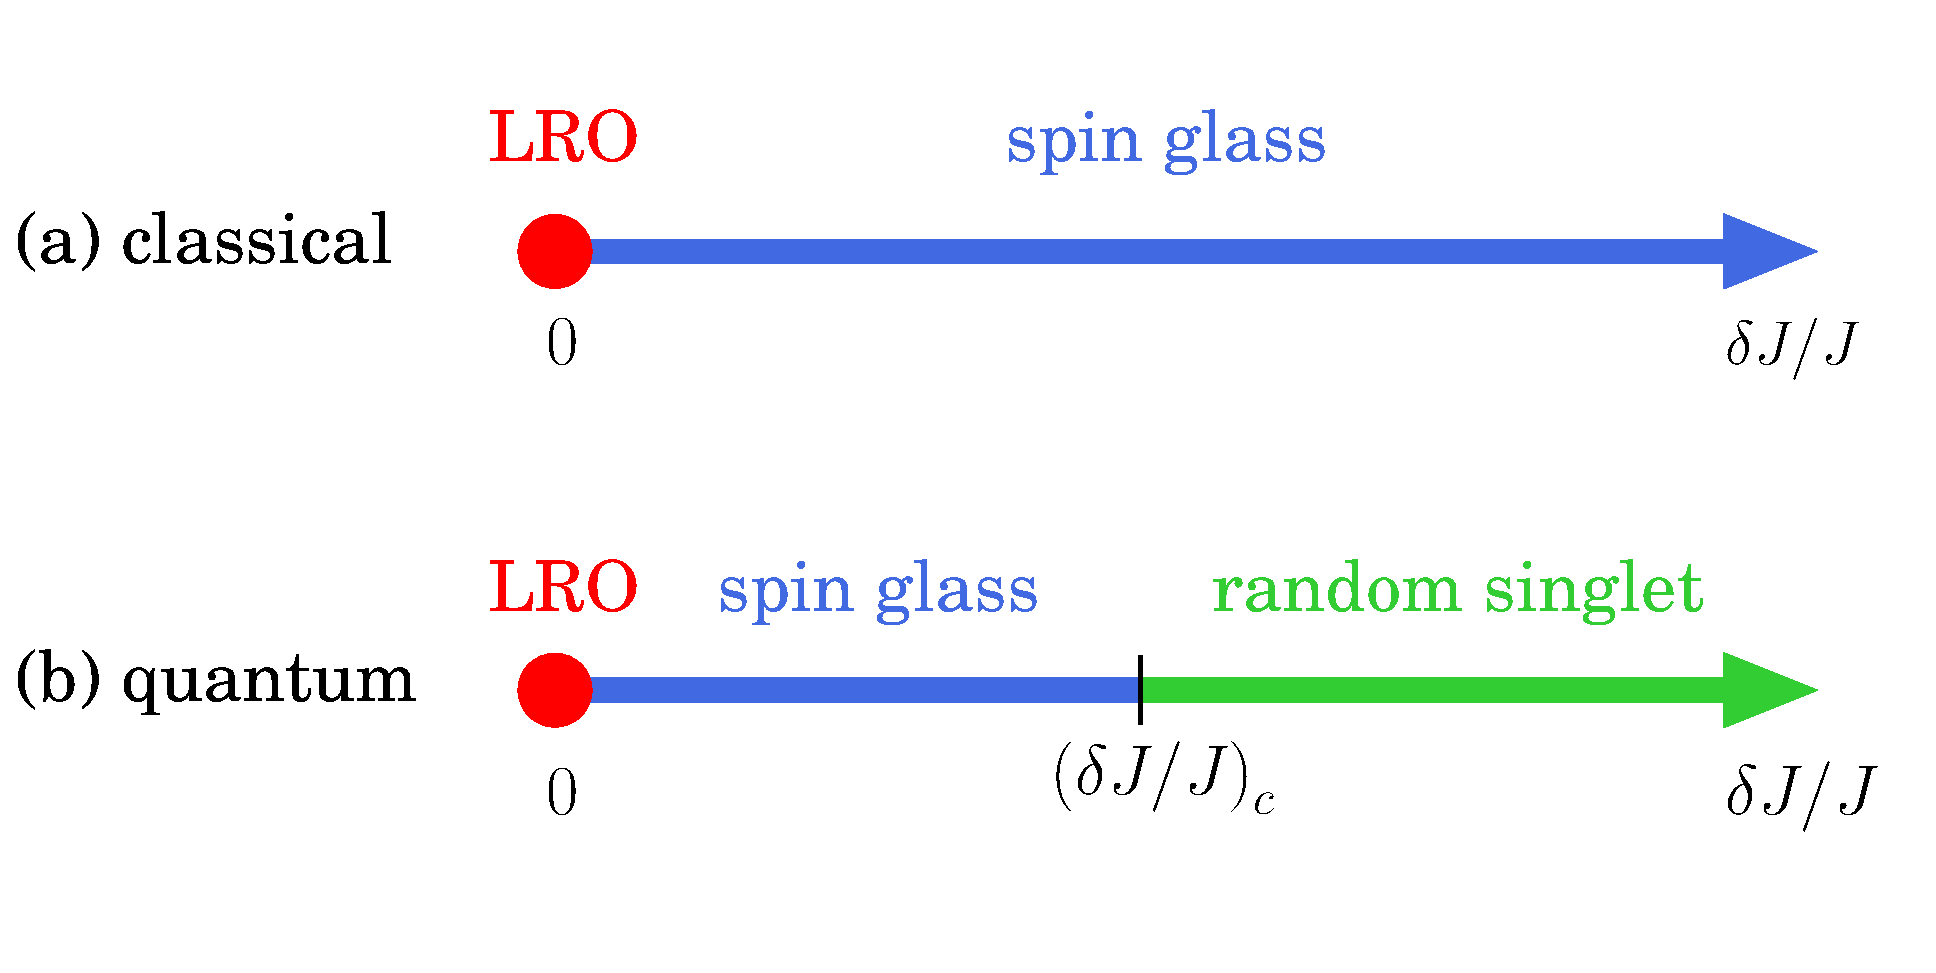
\includegraphics[width=0.95\columnwidth]{fig_pd}
\caption{
Schematic ground-state phase diagram of chiral non-collinear magnets with quenched bond disorder in space dimension $1<d\leq2$, with $\delta J/J$ parameterizing the disorder strength.
%
(a) Classical limit ($S\to\infty$): The LRO of the clean system is destroyed for infinitesimal disorder in favor of a spin glass.
%
(b) Quantum case: The spin glass turns into a random singlet (or valence bond) state at a critical level of disorder (whose numerical value depends on microscopic details).
}
\label{fig:pd}
\end{figure}


%%%%%%%%%%%%%%%%%%%%%%%%%%%%%%%%%%%%%%%%%%%%%%%%%%%%%%%%%%%%%%%%%%%%%%%


\paragraph{Model and general considerations.---}
%
To be specific, we will consider the spin-$S$ triangular-lattice Heisenberg model with nearest-neighbor couplings,
\begin{equation}
\mathcal{H} = \sum_{\langle ij\rangle} J_{ij} \vec{S}_i\cdot\vec{S}_j
\end{equation}
whose ground state in the clean limit, $J_{ij} \equiv J$, displays coplanar spiral $120^\circ$ LRO with propagation wavevector $Q=\pm(4\pi/3,0)$.
%
Importantly, the $120^\circ$ ground state is chiral: Assuming that the spins lie in the $x$-$y$ plane in spin space, the vector chirality $\vec{S}_i\times\vec{S}_j$ for any given directed pair of sites $i$, $j$ can point along either $+\hat{z}$ or $-\hat{z}$, corresponding to the two possible propagation wavevectors and a spontaneously broken Z$_2$ symmetry \cite{braggfoot}. As a result, site inversion symmetry is broken as well, which will play an important role for the defect physics.

We will be interested in the random-bond case where the $J_{ij}$ are (independent) random variables drawn from a bounded distribution. Bond disorder can be made weak either by employing a narrow distribution or by having a small defect concentration, i.e., a situation where most bonds take a value $J$ with only a small concentration of bonds deviating from this.

Our main focus will be on semiclassical spin order -- this is appropriate for the clean system in the presence of LRO, and by continuity also for weakly disordered system. In this regime, quantum effects will only yield quantitative corrections, and we will show explicit results for the classical case, formally $S\to\infty$.
%
Strong quantum effects can be expected to be relevant at large disorder and small $S$: Here, the formation of singlet bonds akin to a random-singlet state has been proposed \cite{kawamura14}; this physics is beyond the scope of this paper.

Most generally, our qualitative results will apply to all two-dimensional magnets with semiclassical non-collinear, but co-planar LRO, both with spontaneous and explicit (i.e. crystallographic) chirality.

%%%%%%%%%%%%%%%%%%%%%%%%%%%%%%%%%%%%%%%%%%%%%%%%%%%%%%%%%%%%%%%%%%%%%%%

\begin{figure}
\begin{centering}
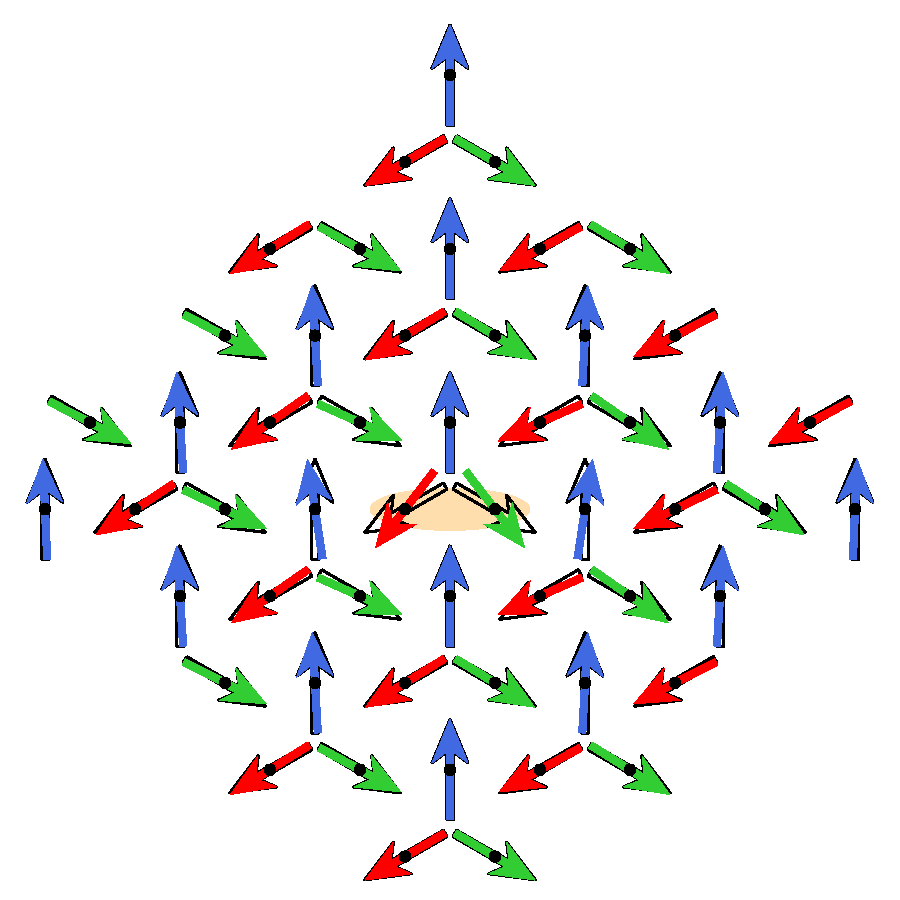
\includegraphics[width=0.5\columnwidth]{config_single_dipole}%
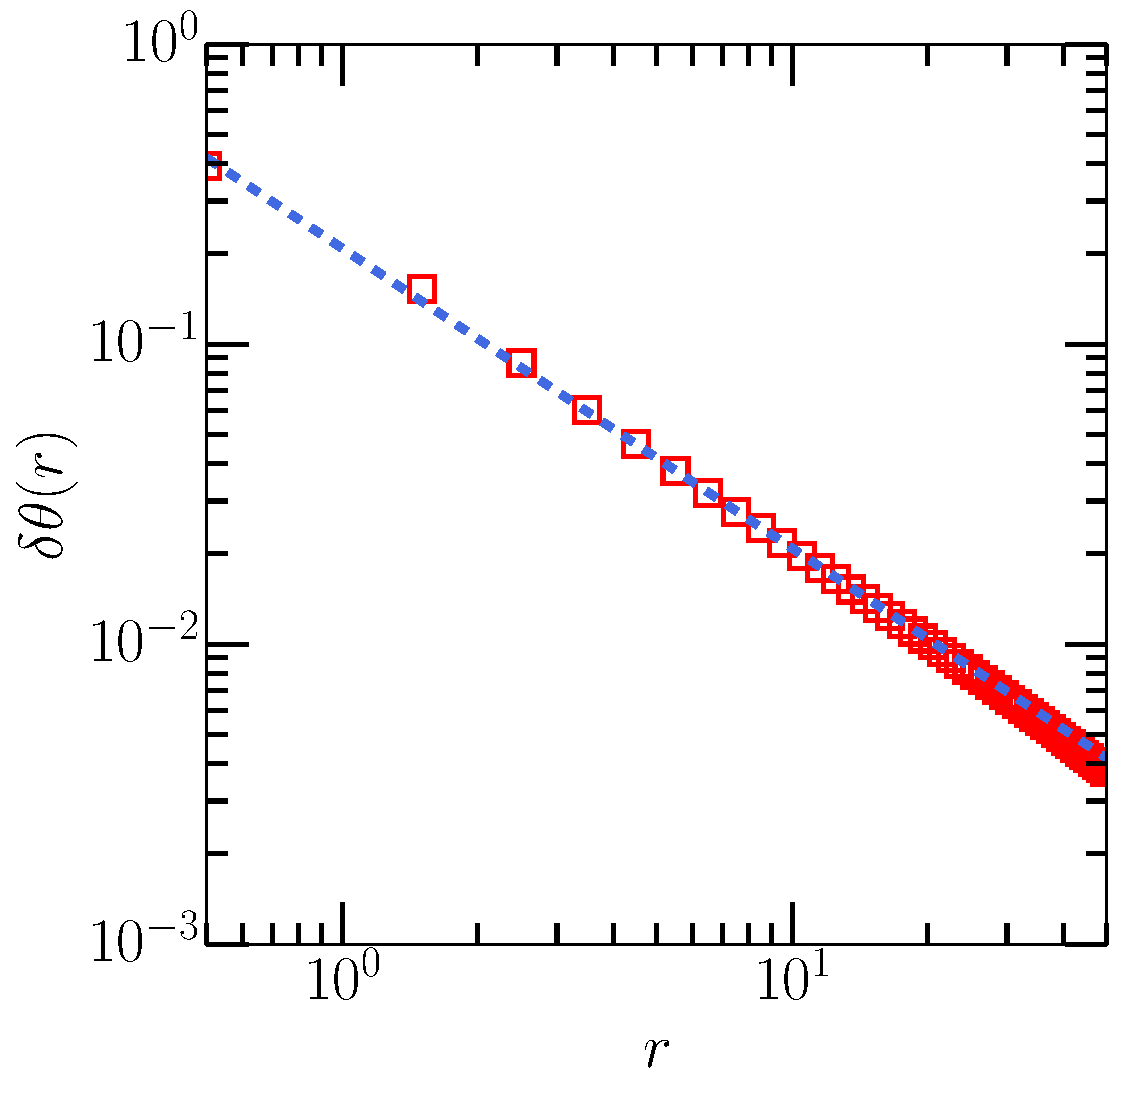
\includegraphics[width=0.5\columnwidth]{th_vs_r}
\end{centering}
\caption{Single bond defect in a triangular-lattice Heisenberg antiferromagnet, with $\delta J=-J$ \eqref{onebond}, i.e., a missing bond.
%
(a) Spin configuration near the defect bond (shaded); the unperturbed $120^\circ$ order is shown in gray.
%
(b) Defect-induced rotation angles $\delta\Theta$ of the spin as function of distance $r$ from the defect. The red line corresponds to a $1/r$ behavior; deviations are large $r$ arise from the finite sample size \todo{$L=100$}. \todo{clarify data inconsistency}
}
\label{fig:single}
\end{figure}


\paragraph{Single bond defect.---}
%
We start by considering a single defect bond in an otherwise homogeneous system,
\begin{equation}
\label{onebond}
J_{ij} = \left\{ \begin{array}{ll} J+\delta J & (i,j)=(0,1), \\ J & \rm{otherwise}. \end{array} \right.
\end{equation}
The presence of the defect locally relieves frustration, leading to a readjustment of the spin directions. This is not unlike the case of a vacancy, studied in some detail in Ref.~\onlinecite{wollny11}.

Numerical results for a bond defect with $\delta J=-J$, embedded in a system of $L^2$ sites with \todo{$L=100$} and periodic boundary conditions, are shown in Fig.~\ref{fig:single}.
%
The spin configuration remains coplanar and can be analyzed in terms of angles $\delta\Theta_i$ which describe the defect-induced in-plane rotation of the spin $\vec{S}_i$ w.r.t. the $120^\circ$ LRO. The Hamiltonian with couplings \eqref{onebond} has site inversion symmetry w.r.t. the center of the defect bond, and we find $\delta\Theta_i$ to be \emph{odd} under this inversion: $\delta\Theta_i$ changes sign at a line perpendicular to the defect bond, has a $p$-wave-like shape and decays proportional to $1/r$ where $r$ is the distance from the defect.
%
Together, this implies that the bond defect acts like a \emph{dipolar} perturbation; this can be contrasted to the case of a vacancy which behaves like an octupole, with an $f$-wave shape and a $1/r^3$ decay of $\delta\Theta_i$ \cite{wollny11}.

The connection between the local release of frustration and the long-range nature and shape of the distortion can be understood at a linear-response level: The frustration is released such that the two spins $0,1$ on the defect bond align more (less) antiparallel compared to the $120^\circ$ state for $\delta J>0$ ($\delta J<0$), respectively. This rotation can be induced by a locally transverse field, $h^\perp \propto \delta J$ acting on $\vec{S}_1$ and $\vec{S}_2$ with opposite signs. It is convenient to work in a local frame of spin coordindates such that the order is uniform along the $\hat{x}$ axis; then the locally transverse field acts as $h^\perp \sum_{j=0}^1 \beta_j S_j^y$ with $\beta_j=(-1)^j$. The long-distance pattern follows as the response of the ordered state to this \emph{local dipolar} field.
%
The relevant transverse susceptibility $\chi^\perp(\vec{q})$ is dominated by the in-plane spin-wave modes whose dispersion is $\w_q\propto|\vec{q}|$ such that $\chi^\perp(\vec{q})\propto 1/q^2$. This yields, in the continuum limit, $\delta\Theta(r) \propto \int d^d q e^{i\vec{q}\cdot\vec{r}} \beta_{\vec{q}} \chi^\perp(\vec{q}) \propto 1/r^{d-1}$ where $\beta_{\vec{q}}\propto q_x$ is the $p$-wave form factor of the local perturbation, thus connecting $p$-wave symmetry and $1/r$ decay in $d=2$ \cite{suppl}.

The fact that a bond defect produces an antisymmetric (or inversion-odd) distortion is intimately connected to the chirality of the clean ground state: The Hamiltonian itself is inversion-even, and a single defect cannot spontaneously break this symmetry. However, the ground state is chiral, with broken inversion symmetry, enabling the defect to produce an odd perturbation. In other words, the ground-state chirality endows the bond defect with a direction, as required for a dipole, and switching the chirality will switch the sign of the dipole.

As an aside, we note that the state with a single bond defect has a finite uniform magnetization, $\mimp$, which takes a non-universal fractional value, similar to the vacancy case \cite{wollny11}. For the bond defect with $\delta J=-J$ we have found \todo{$\mimp = 0.41 S + \mathcal{O}(S^0)$}.

%%%%%%%%%%%%%%%%%%%%%%%%%%%%%%%%%%%%%%%%%%%%%%%%%%%%%%%%%%%%%%%%%%%%%%%

\paragraph{Destruction of long-range order by dipolar fluctuations.---}
%
We now turn to the case of a finite defect concentration and argue that LRO is generically destroyed for $d\leq 2$, adopting an argument originally due to Aharony~\cite{aharony78}. To this end, we assume LRO and employ local rotated frames as above, such that the order is uniform along the $\hat{z}$ axis.
%
We distribute random bonds $J_{ij}$ on the lattice and define $\delta J_{ij}=J_{ij}-J$ where $J=\overline{J_{ij}}$ is the disorder-averaged $J$, such that the disorder strength is parameterized by $\overline{\delta J_{ij}^2} \equiv (\delta J)^2$.
%
The triangular lattice has bonds of three different directions, corresponding to three orientations of dipoles. We define $\hat{e}_{ij}$ as the unit vector connecting $i$ and $j$ \todo{sign convention}. Then $\vec{d}_{ij} \equiv \hat{e}_{ij}\delta J_{ij}/J$ takes the role of a local dipole strength.

For weak randomness, the resulting rotation of an individual spin is proportional to its transverse magnetization in the rotated frame, $\delta\Theta_l = \langle S_{l}^{\perp} \rangle / |\langle S_{l} \rangle|$. It can be estimated using linear response as above
\begin{align}
\left\langle S_{l}^{\perp}\right\rangle = \alpha S
\sum_{\langle ij\rangle} \frac{\delta J_{ij}}{J} \,
\frac{\hat{e}_{ij}\cdot\hat{e}_{l,ij}}{r_{l,ij}^{d-1}}
\end{align}
where $r_{l,ij}$ is the distance between site $l$ and the center of the $ij$ bond, $\hat{e}_{l,ij}$ is the corresponding unit vector, and $\alpha$ a numerical prefactor whose magnitude characterizes the ``dipolar'' susceptibility of the bulk LRO. \todo{adjust prefactor discussion}
%
The disorder-averaged transverse magnetization, $\overline{\langle S_{j}^{\perp}\rangle}$, vanishes because the averaged dipole strength has zero mean. In contrast, the averaged magnetization correlation function is non-zero,
\begin{equation}
\overline{\left\langle {S_{l}^{\perp}}^2\right\rangle } = 3\alpha(\delta J)^{2} S^2 \int{\rm d}^{d}r \,r^{2-2d} \cos^2 \phi_{lr}
\label{fluctint}
\end{equation}
where we have passed to the continuum limit, $\phi_{lr}$ is the polar angle of the line connecting $l$ and $r$, and the summation of the three types of bonds has been performed, see Ref.~\onlinecite{suppl} for details.

The above integral is infrared divergent for $d\leq 2$, such that the local transverse magnetization fluctuations diverge for $d\leq2$: These fluctuations, arising from dipolar bond disorder and transmitted by long-wavelength modes, then destroy the assumed ordered state. For $d>2$ a finite defect concentration is required to destroy order; we will come back to this at the end of the paper.


%%%%%%%%%%%%%%%%%%%%%%%%%%%%%%%%%%%%%%%%%%%%%%%%%%%%%%%%%%%%%%%%%%%%%%%

\paragraph{Incommensurability glass.---}
%
We now discuss the nature of the emerging state without LRO.
%
First, the above argument implies that order is destroyed by dipole-like fluctuations; hence, large fluctuations correspond to anomalously large dipole densities.
%
Second, in order to gain insight into the physics of large dipole densities, let us consider a region of locally uniform non-vanishing dipole density: On the triangular lattice, this is realized if bonds along one direction deviate from those in the others in a correlated fashion, locally realizing an anisotropic triangular Heisenberg magnet \cite{tri_aniso}. \todo{figure?}
%
This is a well-studied model, known to host spiral phases at the classical level, with the ordering wavevector depending continuously on the coupling-constance anisotropy \cite{tri_aniso}. Assuming horizontal bonds of strength $J'$, the ordering wavevector is $\pm(Q_x,Q_y)$ with $Q_x = 2\arccos(1/(4J'/J-2))$ and $Q_y= -(1/\sqrt{3}) \arccos(1/(4J'/J-2))$ for $J'/J>3/4$.
\todo{check, illustrate}

In fact, we can directly relate the dipole density to the wavevector incommensurability:
If we denote the couplings by $J_{1,2,3}$ on the bonds $1,2,3$, with mean $J$, we can define $\vec{d} = \sum_{i=1}^3 (J_i/J) \hat{e}_i$ and find $\vec{Q}-\vec{Q}_0 = \kappa \vec{d}$ where $\vec{Q}_0$ is the ordering wavevector of the isotropic reference system, $Q_0=\pm(4\pi/3,0)$ for the two chiralities. Note that switching the chirality inverts the dipole density $\vec{d}$, but also inverts $\vec{Q}$ and $\vec{Q}_0$.


\begin{figure}
\begin{centering}
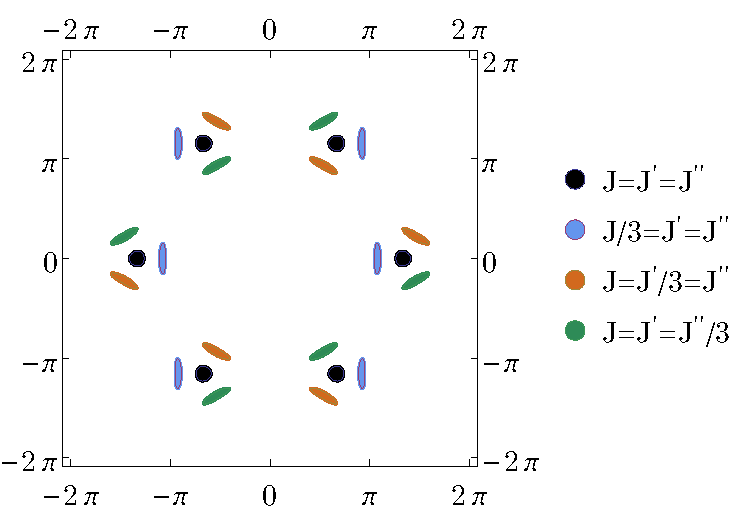
\includegraphics[width=0.9\columnwidth]{anisotropy-Q}%
\end{centering}
\caption{Illustration of the ordering wavevector for the anisotropic triangular-lattice Heisenberg model. The deviation from $\vec{Q}_0=\pm(4\pi/3,0)$ is proportional to the dipole density $\vec{d}$ defined in ...
%
}
\label{fig:vecs}
\end{figure}

We conclude that finite dipole density introduces incommensurability in the spin order.

Taken together, this suggests that a bond-disordered system will display regions (i.e. domains) of locally different incommensurability induced by regions of anomalous dipole density. We term the resulting state in $d\leq 2$, lacking LRO, an \emph{incommensurability glass}. This is a short-range-ordered state with glass-like properties, i.e., random freezing of moments.
%
We note that $d=2$ is below the lower critical dimension for spin-glass order \cite{parisi17}, hence, there will be no thermodynamic glass transition in $d=2$.

We can estimate the correlation length $\xi$ simply by assuming that it provides an infrared cut-off to the integral \eqref{fluctint} by identifying $\xi$ with the domain size $\ell$. The stability condition $\overline{\langle {S_{l}^{\perp}}^2\rangle }=1$ translates into $\xi^{2-d} \propto (J/\delta J)^2$ for $d<2$, while in $d=2$
\begin{equation}
\xi \propto e^{(J/\delta J)^2}\,.
\label{xi}
\end{equation}
We note that the domain picture allows us to connect our considerations with the celebrated arguments by Imry and Ma~\cite{imry_ma}. Consider domains inside which the dipole density is atypically strong, such that the local order adopts a corresponding incommensurability. The energy gain scales as $\delta J\ell^{d/2}$ (as dictated by the central limit theorem). This must be balanced against the domain-wall energy cost: Here, we have sharp domain walls because a local wavevector deviation costs a finite energy. This yields a domain wall energy which scales as $J\ell^{d-1}$. Thus, for $d<2$ it is favorable to break the system into domains of linear size $\ell\gtrsim\left(J/\delta J\right)^{2/(2-d)}$, consistent with the above estimate.


%%%%%%%%%%%%%%%%%%%%%%%%%%%%%%%%%%%%%%%%%%%%%%%%%%%%%%%%%%%%%%%%%%%%%%

\paragraph{Numerical results for finite disorder.---}

\todo{how good are our results? push size?}

\todo{one config - bonds color coded according to cos}

%%%%%%%%%%%%%%%%%%%%%%%%%%%%%%%%%%%%%%%%%%%%%%%%%%%%%%%%%%%%%%%%%%%%%%%

\paragraph{Perturbations: Finite $T$, interlayer coupling, and anisotropies.---}
%
Beyond the idealized model discussed so, a number of effects are important.
%
First, in a strictly two-dimensional SU(2)-symmetric system, the clean-limit LRO is restricted to $T\!=\!0$ due to the Mermin-Wagner theorem. Hence, the clean system is short-range-ordered at any finite $T$, with the thermal correlation length scaling as $\xi_T \propto e^{1/T}$ \todo{polish}. Now, bond disorder limits the correlation length according to Eq.~\eqref{xi}, which defines a disorder-dependent crossover temperature which scales linearly with the disorder level, $T^\ast \propto (\delta J)^2/J$, below which the system settles into its $T\!=\!0$ glassy state.
%
Second, a small but finite interlayer coupling will render the system three-dimensional at sufficiently low temperature, leading to finite-$T$ LRO which is also stable against weak bond disorder. As a result, LRO is destroyed in favor of a glassy state only beyond a critical level of disorder which scales linearly with the interlayer coupling \todo{refine argument: integral cut-off}. $J_\perp \propto (\delta J)^2/J$.
%
Third, if SU(2) is broken down to a discrete symmetry at the Hamiltonian level, the clean system acquires a gap, again stabilizing finite-$T$ LRO which is stable against weak bond disorder. Here, the critical level of disorder beyond which LRO is destroyed, scales linearly with the gap \todo{refine argument: integral cut-off}, for details see Ref.~\onlinecite{suppl}.

We also note that a strictly two-dimensional system will not display a finite-temperature glass transition, as $d\!=\!2$ is known to be the lower critical dimension for spin-glass order.
...
\todo{can we come up with a proposal to **tune** glass transition?}

\todo{phase diagram $T$ vs $\Delta$ for finite $J_\perp$?}
%%%%%%%%%%%%%%%%%%%%%%%%%%%%%%%%%%%%%%%%%%%%%%%%%%%%%%%%%%%%%%%%%%%%%%%

\paragraph{Quantum effects.---}
%
So far our analysis was based on semiclassical spin order. It is strictly valid for $S\to\infty$, but qualitatively also applies to finite $S$: $1/S$ corrections to observables can be calculated and are generically non-singular at $T\!=\!0$ \cite{wollny11,suppl}. However, for small $S$ the physics can change; in particular, local spin order can be destroyed in favor of singlet formation.
%
If magnetic LRO is present in the clean limit, then a finite amount of bond disorder can lead to the suppression of local order via the emergence of a disorder-dominated valence-bond state, similar to the celebrated random-singlet state in one dimension \todo{cite}. In fact, the emergence of such a state has been proposed on the basis of numerical simulations for the bond-disordered Heisenberg model both on the triangular and honeycomb lattices.
%
Together with our insight that infinitesimal bond disorder destroys non-collinear LRO in favor of a spin glass, we conjecture the phase diagram in Fig. xxx(b), where the glass gives way to a random-singlet state at large disorder.

%%%%%%%%%%%%%%%%%%%%%%%%%%%%%%%%%%%%%%%%%%%%%%%%%%%%%%%%%%%%%%%%%%%%%%%

\paragraph{Conclusions.---}
%
Combining different analytical arguments, we have shown that random-bond defects destroy long-range magnetic order in the ground state of two-dimensional non-collinear antiferromagnets with SU(2) spin symmetry. The key insight, demonstrated explicitly for the triangular-lattice Heisenberg model, is that individual bond defects induce a dipolar distortion with $1/r$ decay of the spin background. As a result, a finite concentration of defects produces fluctuating incommensurabilities which destabilize LRO even for weak disorder in favor of a spin-glass state.

Remarkably, the effect of random site dilution is much weaker: Vacancies induce an octupolar distortion with $1/r^3$ decay \cite{wollny11}, and LRO is stable against a small vacancy concentration because the integral corresponding to Eq.~\eqref{fluctint} is {\em not} divergent.

Our analysis shows that none of the two cases can be described as random-mass disorder in the relevant low-energy field theory for the ordered state, because this would miss the defect-induced random transverse fields. This underlines a fundamental difference between the present non-collinear magnets and their unfrustrated collinear counterparts, where both random-bond disorder and site dilution correspond to random-mass terms in the field theory.

We expect our ideas to motivate further studies into different types of quenched disorder in weakly frustrated magnets. Investigations for semiclassical non-coplanar order are underway.

%%%%%%%%%%%%%%%%%%%%%%%%%%%%%%%%%%%%%%%%%%%%%%%%%%%%%%%%%%%%%%%%%%%%%%%

\begin{acknowledgments}
We are grateful to E. Andrade, W. Brenig, J. A. Hoyos, S. Rachel, and S. Trebst for instructive discussions and collaborations on related work.
%
This research was supported by the Deutsche Forschungsgemeinschaft (DFG) via GRK 1621 and project A01 of SFB 1143.
\end{acknowledgments}

%%%%%%%%%%%%%%%%%%%%%%%%%%%%%%%%%%%%%%%%%%%%%%%%%%%%%%%%%%%%%%%%%%%%%%%

\begin{thebibliography}{99}

\bibitem{starykh13}
%Unusual ordered phases of highly frustrated magnets: a review
O. A. Starykh,
Rep. Prog. Phys. {\bf 78}, 052502 (2015).

\bibitem{villain79}
J. Villain,
Z. Phys. B \textbf{33}, 31 (1979).

\bibitem{chalker07}
%Spin Freezing in Geometrically Frustrated Antiferromagnets with Weak Disorder
T. E. Saunders and J. T. Chalker,
Phys. Rev. Lett. \textbf{98}, 157201 (2007).

\bibitem{chalker10}
% Spin glass transition in geometrically frustrated antiferromagnets with weak disorder
A. Andreanov, J. T. Chalker, T. E. Saunders, and D. Sherrington,
Phys. Rev. B \textbf{81}, 014406 (2010).

\bibitem{zhito14}
V. S. Maryasin and M. E. Zhitomirsky,
Phys. Rev. B \textbf{90}, 094412 (2014).

\bibitem{henley89}
C. L. Henley,
Phys. Rev. Lett. \textbf{62}, 2056 (1989).

\bibitem{igloi05}
% Strong disorder RG approach of random systems
F. Igloi and C. Monthus,
Phys. Rep. \textbf{412}, 277 (2005)

\bibitem{aharony78}
A. Aharony,
Solid State Commun. \textbf{28}, 667 (1978).

\bibitem{fischer}
K. H. Fischer and J. A. Hertz, \emph{Spin Glasses}
(Cambridge University Press, Cambridge, 1991).

\bibitem{imry_ma}
Y. Imry and S.-k. Ma,
Phys. Rev. Lett. \textbf{35}, 1399 (1975).

\bibitem{wollny11}
A. Wollny, L. Fritz, and M. Vojta,
% Fractional impurity moments in two-dimensional non-collinear magnets,
Phys. Rev. Lett. {\bf 107}, 137204 (2011).

\bibitem{wollny12}
A. Wollny, E. C. Andrade, and M. Voj\-ta,
% Singular field response and singular screening of vacancies in antiferromagnets,
Phys. Rev. Lett. {\bf 109}, 177203 (2012).

\bibitem{kawamura14}
%Quantum spin-liquid behavior in the spin-1/2 random Heisenberg antiferromagnet on the triangular lattice
K. Watanabe, H. Kawamura, H. Nakano, and T. Sakai,
J. Phys. Soc. Jpn. \textbf{83}, 034714 (2014).

\bibitem{braggfoot}
The static spin structure factor of the 120$^\circ$ LRO displays Bragg peaks at both $\pm(4\pi/3,0)$, i.e., is insensitive to chirality.

\bibitem{suppl}
See supplementary material at XXX for details on the linear-response calculations, the relation between dipole density and incommensurability, and further numerical results.

\bibitem{tri_aniso}
J. Villain, J. Phys. Chem. Solids \textbf{11}, 303 (1959);
A. Yoshimori, J. Phys. Soc. Jpn. \textbf{14}, 807 (1959).

\bibitem{parisi17}
A. Maiorano and G. Parisi,
%New support for the value 5/2 for the spin glass lower critical dimension at zero magnetic field
preprint arXiv:1711.05590.

\end{thebibliography}

\end{document}
